\section{Aquisi��o dos dados para identifica��o do sistema}
\label{sec:get_data}
%===============================================================================

O sistema apresentado na se��o (\ref{sec:modelling}) � a descri��o matem�tica para
a planta do sistema, e a fun��o de transfer�ncia utilizada, � a que descreve a
posi��o angular do sistema com rela��o a tens�o aplicada sobre os terminais do motor.

Na pr�tica o que o que foi utilizado � um sistema como o apresentado na Figura (\ref{fig:sys_pid})
onde a planta que se quer identificar esta sendo controlada por um controlador do tipo PID
(Proporcional, integral diferencial) \cite{Ogata}. Onde aplica-se uma referencia a o sistema 
deve seguir esta referencia.

\begin{figure}[htbp]
	\center
	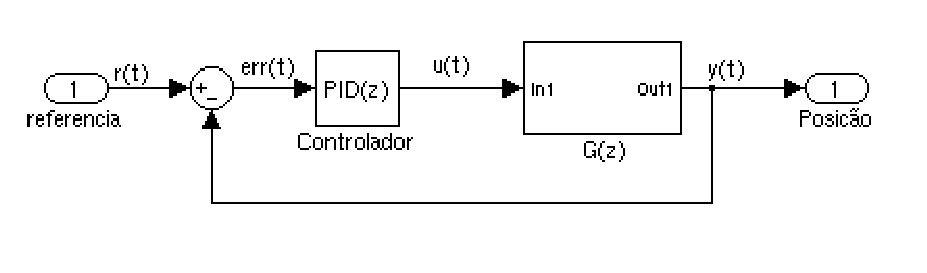
\includegraphics[width=0.98\columnwidth]{figures/sys_pid.eps}
	\caption{Representa��o do sistema utilizado para a coleta dos dados a serem utilizados no 
	processo de estimativa dos par�metros da fun��o $G(q)$.}
	\label{fig:sys_pid}
\end{figure}

Com este sistema foi poss�vel fazer coleta dos dados dos sinais $r(t)$, $y(t)$ al�m do sinal
$u(t)$ que � o sinal de entrada da planta a ser identificada.

Com estes dados � poss�vel proceder de duas maneiras distintas para estimar os valores dos 
par�metros de $G(q)$, � poss�vel apenas utilizar os sinais $r(t)$ e $y(t)$ e adicionar ao modelo
apresentado na se��o (\ref{sec:modelling}) o modelo do controlador PID, j� que este tem um modelo
conhecido e seus par�metros foram previamente escolhidos (antes da simula��o).

Outra maneira poss�vel � utilizar apenas os sinais $u(t)$ e $y(t)$, desta forma pode-se ignorar a
exist�ncia do controlador PID, e utilizar o m�todo desejado, apenas com o modelo do processo.

